%%%%%%%%%%%%%%%%%%%%%%%%%%%%%%%%%%%%%%%%%%%%%%%%%%%%%%%%%%%%%%%%%%%%%%%%%%%%%%%%%%%%%%%%%%
% Data selection and optimization
%%%%%%%%%%%%%%%%%%%%%%%%%%%%%%%%%%%%%%%%%%%%%%%%%%%%%%%%%%%%%%%%%%%%%%%%%%%%%%%%%%%%%%%%%%
\subsection{Overview}

The selection follows the sequence developed for the
$\bar{p}\Lambda^0$ analysis. The stages, each optimized before the next
is applied, are:
%
\begin{enumerate}
    \item preselection: single-candidate requirements and the
          \mes/\DeltaE\ fitting region (this section);
    \item $\Lambda^0$ (and $\Lambda_c^+$, $K_S^0$) purity requirements:
          flight-length significance and mass windows;
    \item particle-identification (PID) selectors, optimized with the
          Punzi figure of merit;
    \item an antibaryon veto;
    \item a multilayer-perceptron classifier built on event-shape
          variables, with its output requirement optimized using a
          \DeltaE-sideband background estimate.
\end{enumerate}
%
The dominant backgrounds are continuum $q\bar{q}$ production (with
$c\bar{c}$ and $u\bar{u}/d\bar{d}/s\bar{s}$ contributing roughly equally
after preselection) and combinatorial $\Lambda$ candidates in $\BB$
events. This section documents the preselection and the diagnostic
distributions used to validate the samples; the optimization of stages
2--5 will be documented in subsequent sections as it is completed.

\subsection{Candidate reconstruction and multiplicities}

For $\Bz \rightarrow \Lambda^0\Lambda^0$, $B$ candidates are formed from
two $\Lambda^0 \rightarrow p \pi^-$ candidates. For
$\Bu \rightarrow \Lambda_c^+\Lambda^0$, $B$ candidates are formed from a
$\Lambda_c^+$ candidate (reconstructed in the four modes described
below) and a $\Lambda^0 \rightarrow p \pi^-$ candidate.

Figure~\ref{fig:multiplicities} shows the numbers of $B$, $\Lambda^0$,
and (where applicable) $\Lambda_c^+$ candidates per event before any
selection. The combinatorics of the two channels are very different: in
the $\Lambda^0\Lambda^0$ channel almost all events contain a single $B$
candidate, while in the $\Lambda_c^+\Lambda^0$ channel the many
$\Lambda_c^+$ reconstruction combinations produce up to $\sim$60 $B$
candidates in a single event.

\begin{figure}[tbp]
    \centering
    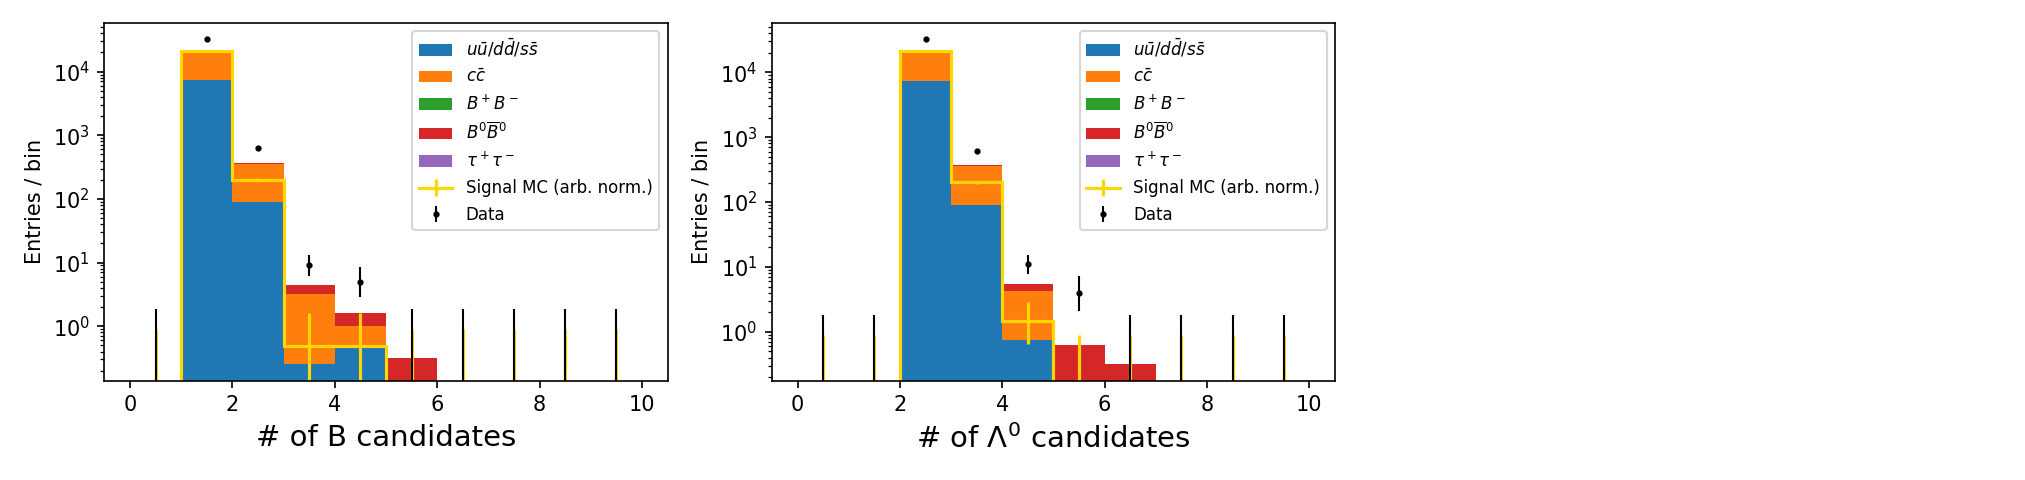
\includegraphics[width=0.95\textwidth]{figures/Lam0Lam0/diagnostics_cut0_multiplicity.png}
    
\includegraphics[width=0.95\textwidth]{figures/Lam0LamC/diagnostics_cut0_multiplicity.png}
    \caption{Candidate multiplicities per event before any selection,
    for $\Bz \rightarrow \Lambda^0\Lambda^0$ (top) and
    $\Bu \rightarrow \Lambda_c^+\Lambda^0$ (bottom). Stacked histograms
    are luminosity-weighted background MC; points are the blinded
    collision data; the line is signal MC with arbitrary normalization.}
    \label{fig:multiplicities}
\end{figure}

\subsection{Preselection and diagnostic cutflow}

The preselection used for the diagnostic studies consists of:
%
\begin{itemize}
    \item[\bf 1.] {\bf single-candidate requirement:} exactly one $B$
        candidate, and exactly the expected number of composite
        daughters (two $\Lambda^0$ for $\Bz \rightarrow
        \Lambda^0\Lambda^0$; one $\Lambda_c^+$ and one $\Lambda^0$ for
        $\Bu \rightarrow \Lambda_c^+\Lambda^0$);
    \item[\bf 2.] {\bf fitting region:} the $B$ candidate lies within
        the \mes/\DeltaE\ fitting region defined in
        Section~\ref{sec:blinding}.
\end{itemize}
%
Tables~\ref{tab:cutflowLamLam} and \ref{tab:cutflowLamLamC} give the
numbers of events passing each requirement for all samples. The
single-candidate requirement retains
essentially all signal in the $\Lambda^0\Lambda^0$ channel
(\LamLamCutflowSignalCutOne\ of \LamLamCutflowSignalCutZero\ events)
but only about half in the $\Lambda_c^+\Lambda^0$ channel
(\LamLamCCutflowSignalCutOne\ of \LamLamCCutflowSignalCutZero); the
mode-dependence of this loss is quantified below.

% AUTO-GENERATED -- DO NOT EDIT BY HAND
\begin{table}[h]
\caption{Numbers of events (raw, unweighted) passing the diagnostic cuts for the $B^0 \to \Lambda^0 \Lambda^0$ channel.}
\label{tab:cutflowLamLam}
\centering
\small
\begin{tabular}{llrrrrrrr}
\toprule
Cut & Description & Signal MC & $u\bar{u}/d\bar{d}/s\bar{s}$ & $c\bar{c}$ & $B^+B^-$ & $B^0\overline{B}^0$ & $\tau^+\tau^-$ & data \\
\midrule
0 & no cut & 44\,755 & 29\,798 & 28\,500 & 145 & 305 & 155 & 33\,278 \\
1 & single candidate & 44\,336 & 29\,439 & 27\,953 & 137 & 277 & 153 & 32\,229 \\
2 & single cand. + fit region & 44\,163 & 7\,503 & 7\,024 & 42 & 71 & 26 & 7\,831 \\
\bottomrule
\end{tabular}
\end{table}


% AUTO-GENERATED -- DO NOT EDIT BY HAND
\begin{table}[h]
\caption{Numbers of events (raw, unweighted) passing the diagnostic cuts for the $B^+ \to \Lambda_c^+ \Lambda^0$ channel.}
\label{tab:cutflowLamLamC}
\centering
\small
\begin{tabular}{llrrrrrrr}
\toprule
Cut & Description & Signal MC & $u\bar{u}/d\bar{d}/s\bar{s}$ & $c\bar{c}$ & $B^+B^-$ & $B^0\overline{B}^0$ & $\tau^+\tau^-$ & data \\
\midrule
0 & no cut & 112\,491 & 53\,593 & 94\,837 & 12\,292 & 13\,637 & 40 & 124\,962 \\
1 & single candidate & 57\,497 & 16\,183 & 16\,542 & 1\,257 & 1\,098 & 15 & 22\,531 \\
2 & single cand. + fit region & 56\,213 & 3\,345 & 3\,470 & 305 & 301 & 1 & 4\,114 \\
\bottomrule
\end{tabular}
\end{table}


\subsection{$\Lambda_c^+$ decay modes}
\label{sec:lambdacmodes}

The $\Lambda_c^+$ signal MC was generated in four decay modes in equal
amounts, and candidates are reconstructed in all four. Each candidate is
classified using the number of $\Lambda_c^+$ daughters and the identity
of the first daughter:
%
\begin{center}
\begin{tabular}{clcc}
\hline
Mode & Decay & $n_{\rm daughters}$ & first daughter \\
\hline
1 & $p K^- \pi^+$               & 3 & $p$ \\
2 & $p K_S^0$                   & 2 & $p$ \\
3 & $p K_S^0 \pi^+\pi^-$        & 4 & $p$ \\
4 & $\Lambda^0 \pi^+\pi^+\pi^-$ & 4 & $\Lambda^0$ \\
\hline
\end{tabular}
\end{center}

Table~\ref{tab:lambdacmodes} shows the fraction of signal-MC
$\Lambda_c^+$ candidates in each mode, before any selection and after
the single-candidate requirement. Before cuts the four modes appear in
comparable amounts. After the single-candidate requirement, however,
mode 4 is eliminated (\LamLamCModeFracFourSingleCandPct\%): its
$\Lambda^0$ daughter enters the same candidate collection as the
$\Lambda^0$ from the $B$ decay, so these events have at least two
$\Lambda^0$ candidates and fail the $n_{\Lambda^0} = 1$ requirement.
%
\textbf{The treatment of the single-candidate requirement in the
$\Lambda_c^+\Lambda^0$ channel is therefore an open design decision}; it
will be revisited once the PID and purity requirements are in place and
the multiplicity of surviving candidates is known.

% AUTO-GENERATED -- DO NOT EDIT BY HAND
\begin{table}[h]
\caption{Fractions of $\Lambda_c^+$ candidates in signal MC reconstructed in each decay mode, before any cuts and after the single-candidate requirement. The suppression of mode 4 by the $n_{\Lambda^0} = 1$ requirement is discussed in the text.}
\label{tab:lambdacmodes}
\centering
\begin{tabular}{clrr}
\toprule
Mode & Decay & no cut [\%] & single cand. [\%] \\
\midrule
1 & $p K^- \pi^+$ & 31.7 & 40.0 \\
2 & $p K_S^0$ & 22.9 & 41.1 \\
3 & $p K_S^0 \pi^+ \pi^-$ & 22.2 & 19.0 \\
4 & $\Lambda^0 \pi^+ \pi^+ \pi^-$ & 23.2 & 0.0 \\
\bottomrule
\end{tabular}
\end{table}


Figure~\ref{fig:lambdac_mode_split} shows the \mes, \DeltaE, and
$\Lambda_c^+$ mass distributions of signal MC separated by decay mode;
Figure~\ref{fig:lamc_specific} shows the flight-significance
distributions of the $\Lambda^0$ separated by parentage (direct $B$
daughter vs.\ daughter of the $\Lambda_c^+$), the $\Lambda_c^+$ flight
significance, and the $K_S^0$ pre-fit mass and flight significance.

\begin{figure}[tbp]
    \centering
    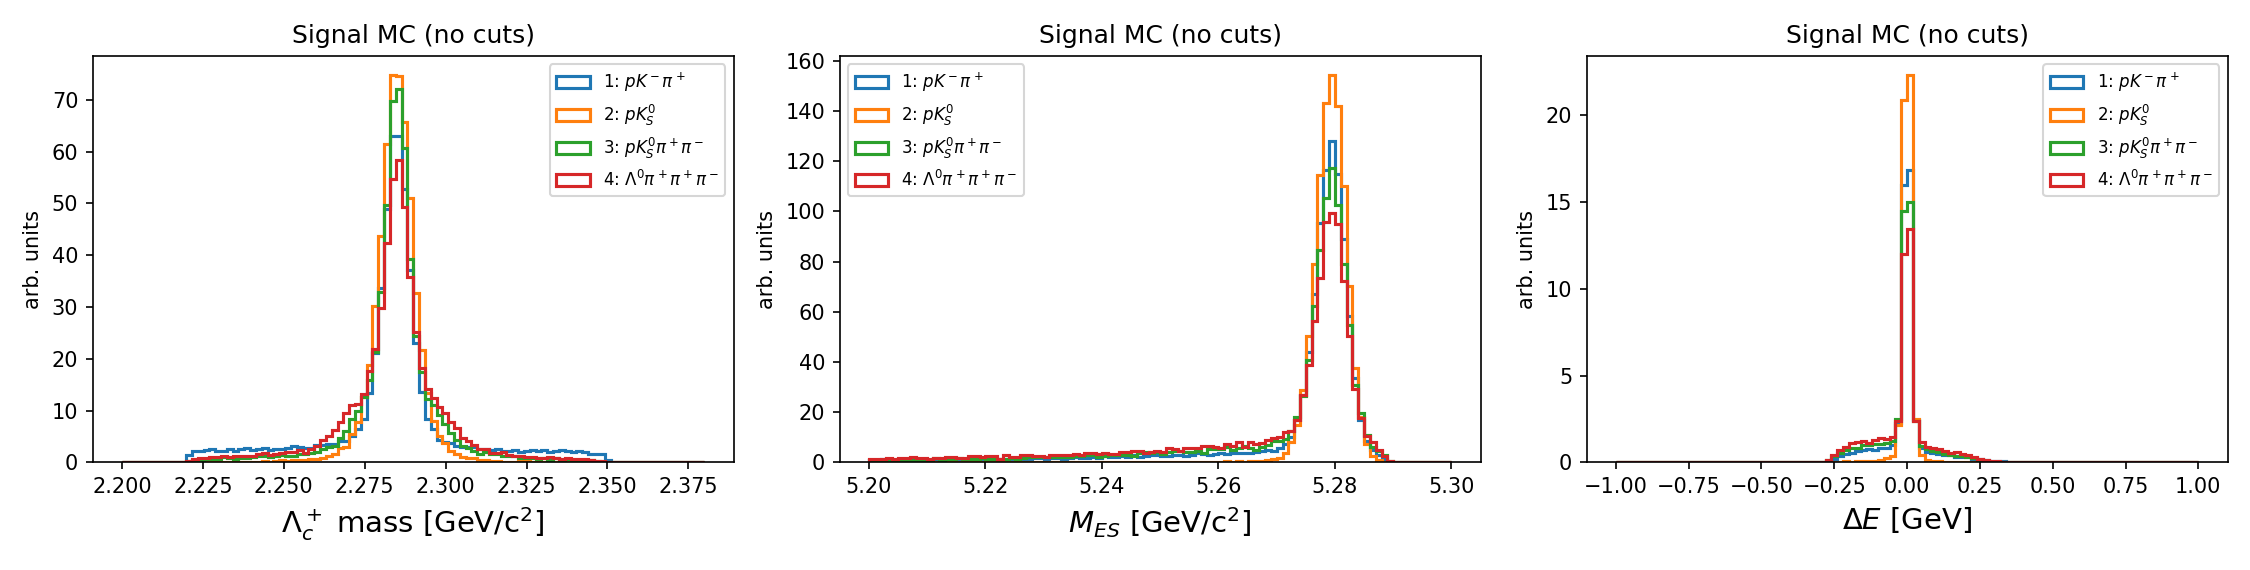
\includegraphics[width=0.99\textwidth]{figures/Lam0LamC/lambdac_mode_split.png}
    \caption{Signal-MC distributions (area-normalized, before any
    selection) separated by $\Lambda_c^+$ decay mode: $\Lambda_c^+$ mass
    (left), \mes\ (center), and \DeltaE\ (right).}
    \label{fig:lambdac_mode_split}
\end{figure}

\begin{figure}[tbp]
    \centering
    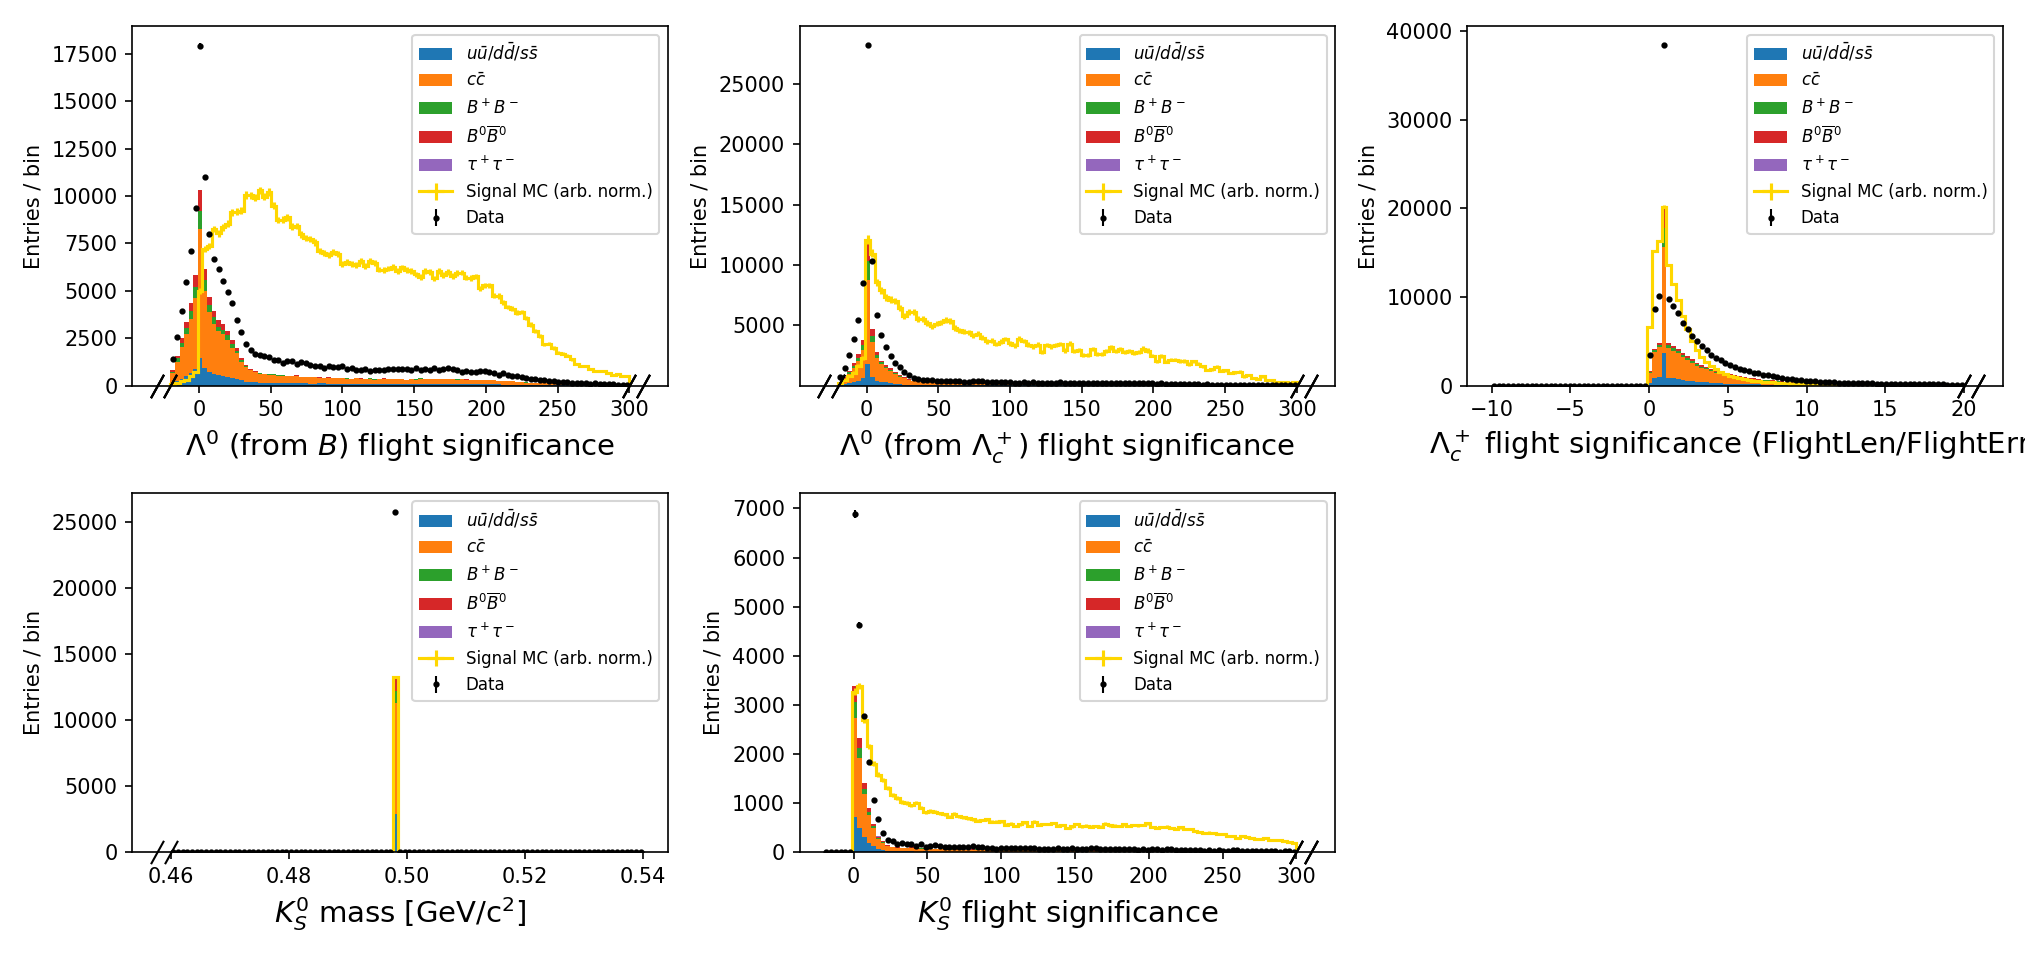
\includegraphics[width=0.99\textwidth]{figures/Lam0LamC/diagnostics_cut0_lamc_specific.png}
    \caption{$\Lambda_c^+\Lambda^0$ channel, before any selection:
    flight significance of $\Lambda^0$ candidates that are direct $B$
    daughters and those used inside a $\Lambda_c^+$; $\Lambda_c^+$
    flight significance; $K_S^0$ pre-fit mass and flight significance.
    Stacked histograms are luminosity-weighted background MC; points are
    blinded collision data; the line is signal MC with arbitrary
    normalization.}
    \label{fig:lamc_specific}
\end{figure}

\subsection{Diagnostic distributions}

Figures~\ref{fig:kinematics_LamLam} and \ref{fig:kinematics_LamLamC}
show the candidate kinematic distributions (\mes, \DeltaE, candidate
masses, and flight quantities) after the single-candidate requirement,
and Figures~\ref{fig:eventshape_LamLam} and \ref{fig:eventshape_LamLamC}
show the event-shape variables that are candidates for the multivariate
classifier. The background MC describes the shapes of the data well. An
overall normalization offset of order a factor of two, also observed in
the $\bar{p}\Lambda^0$ analysis, is visible in some distributions; the
analysis does not rely on the absolute background normalization from MC,
as the background estimate is taken from data sidebands.

\begin{figure}[tbp]
    \centering
    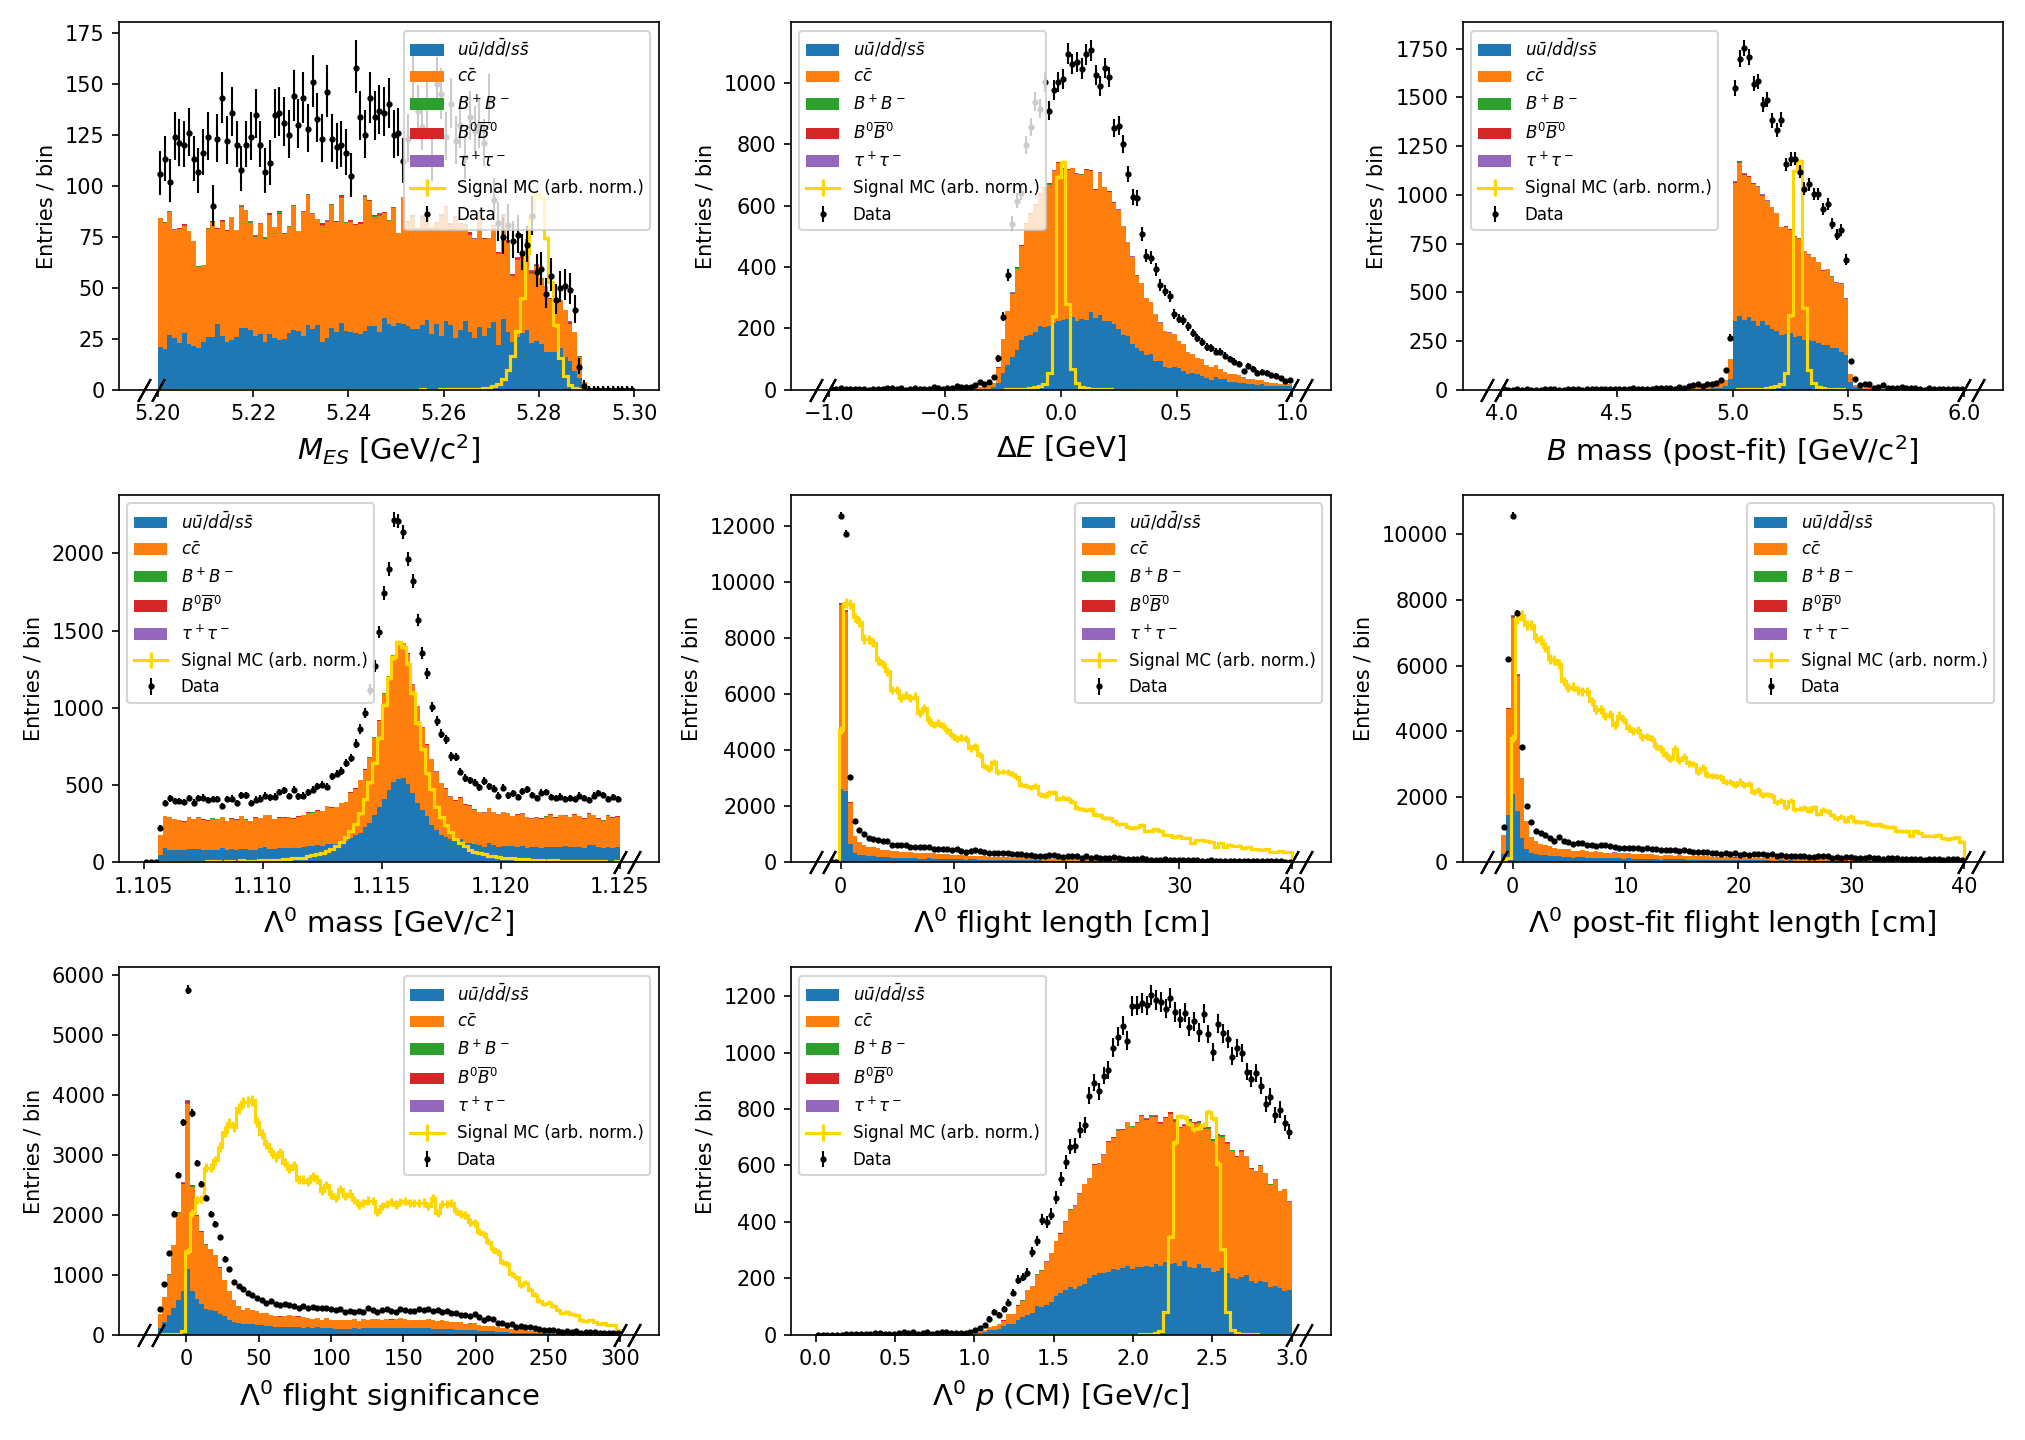
\includegraphics[width=0.99\textwidth]{figures/Lam0Lam0/diagnostics_cut1_kinematics.png}
    \caption{Candidate kinematic distributions for
    $\Bz \rightarrow \Lambda^0\Lambda^0$ after the single-candidate
    requirement. Stacked histograms are luminosity-weighted background
    MC; points are blinded collision data; the line is signal MC with
    arbitrary normalization.}
    \label{fig:kinematics_LamLam}
\end{figure}

\begin{figure}[tbp]
    \centering
    
\includegraphics[width=0.99\textwidth]{figures/Lam0LamC/diagnostics_cut1_kinematics.png}
    \caption{Same as Figure~\ref{fig:kinematics_LamLam} for
    $\Bu \rightarrow \Lambda_c^+\Lambda^0$.}
    \label{fig:kinematics_LamLamC}
\end{figure}

\begin{figure}[tbp]
    \centering
    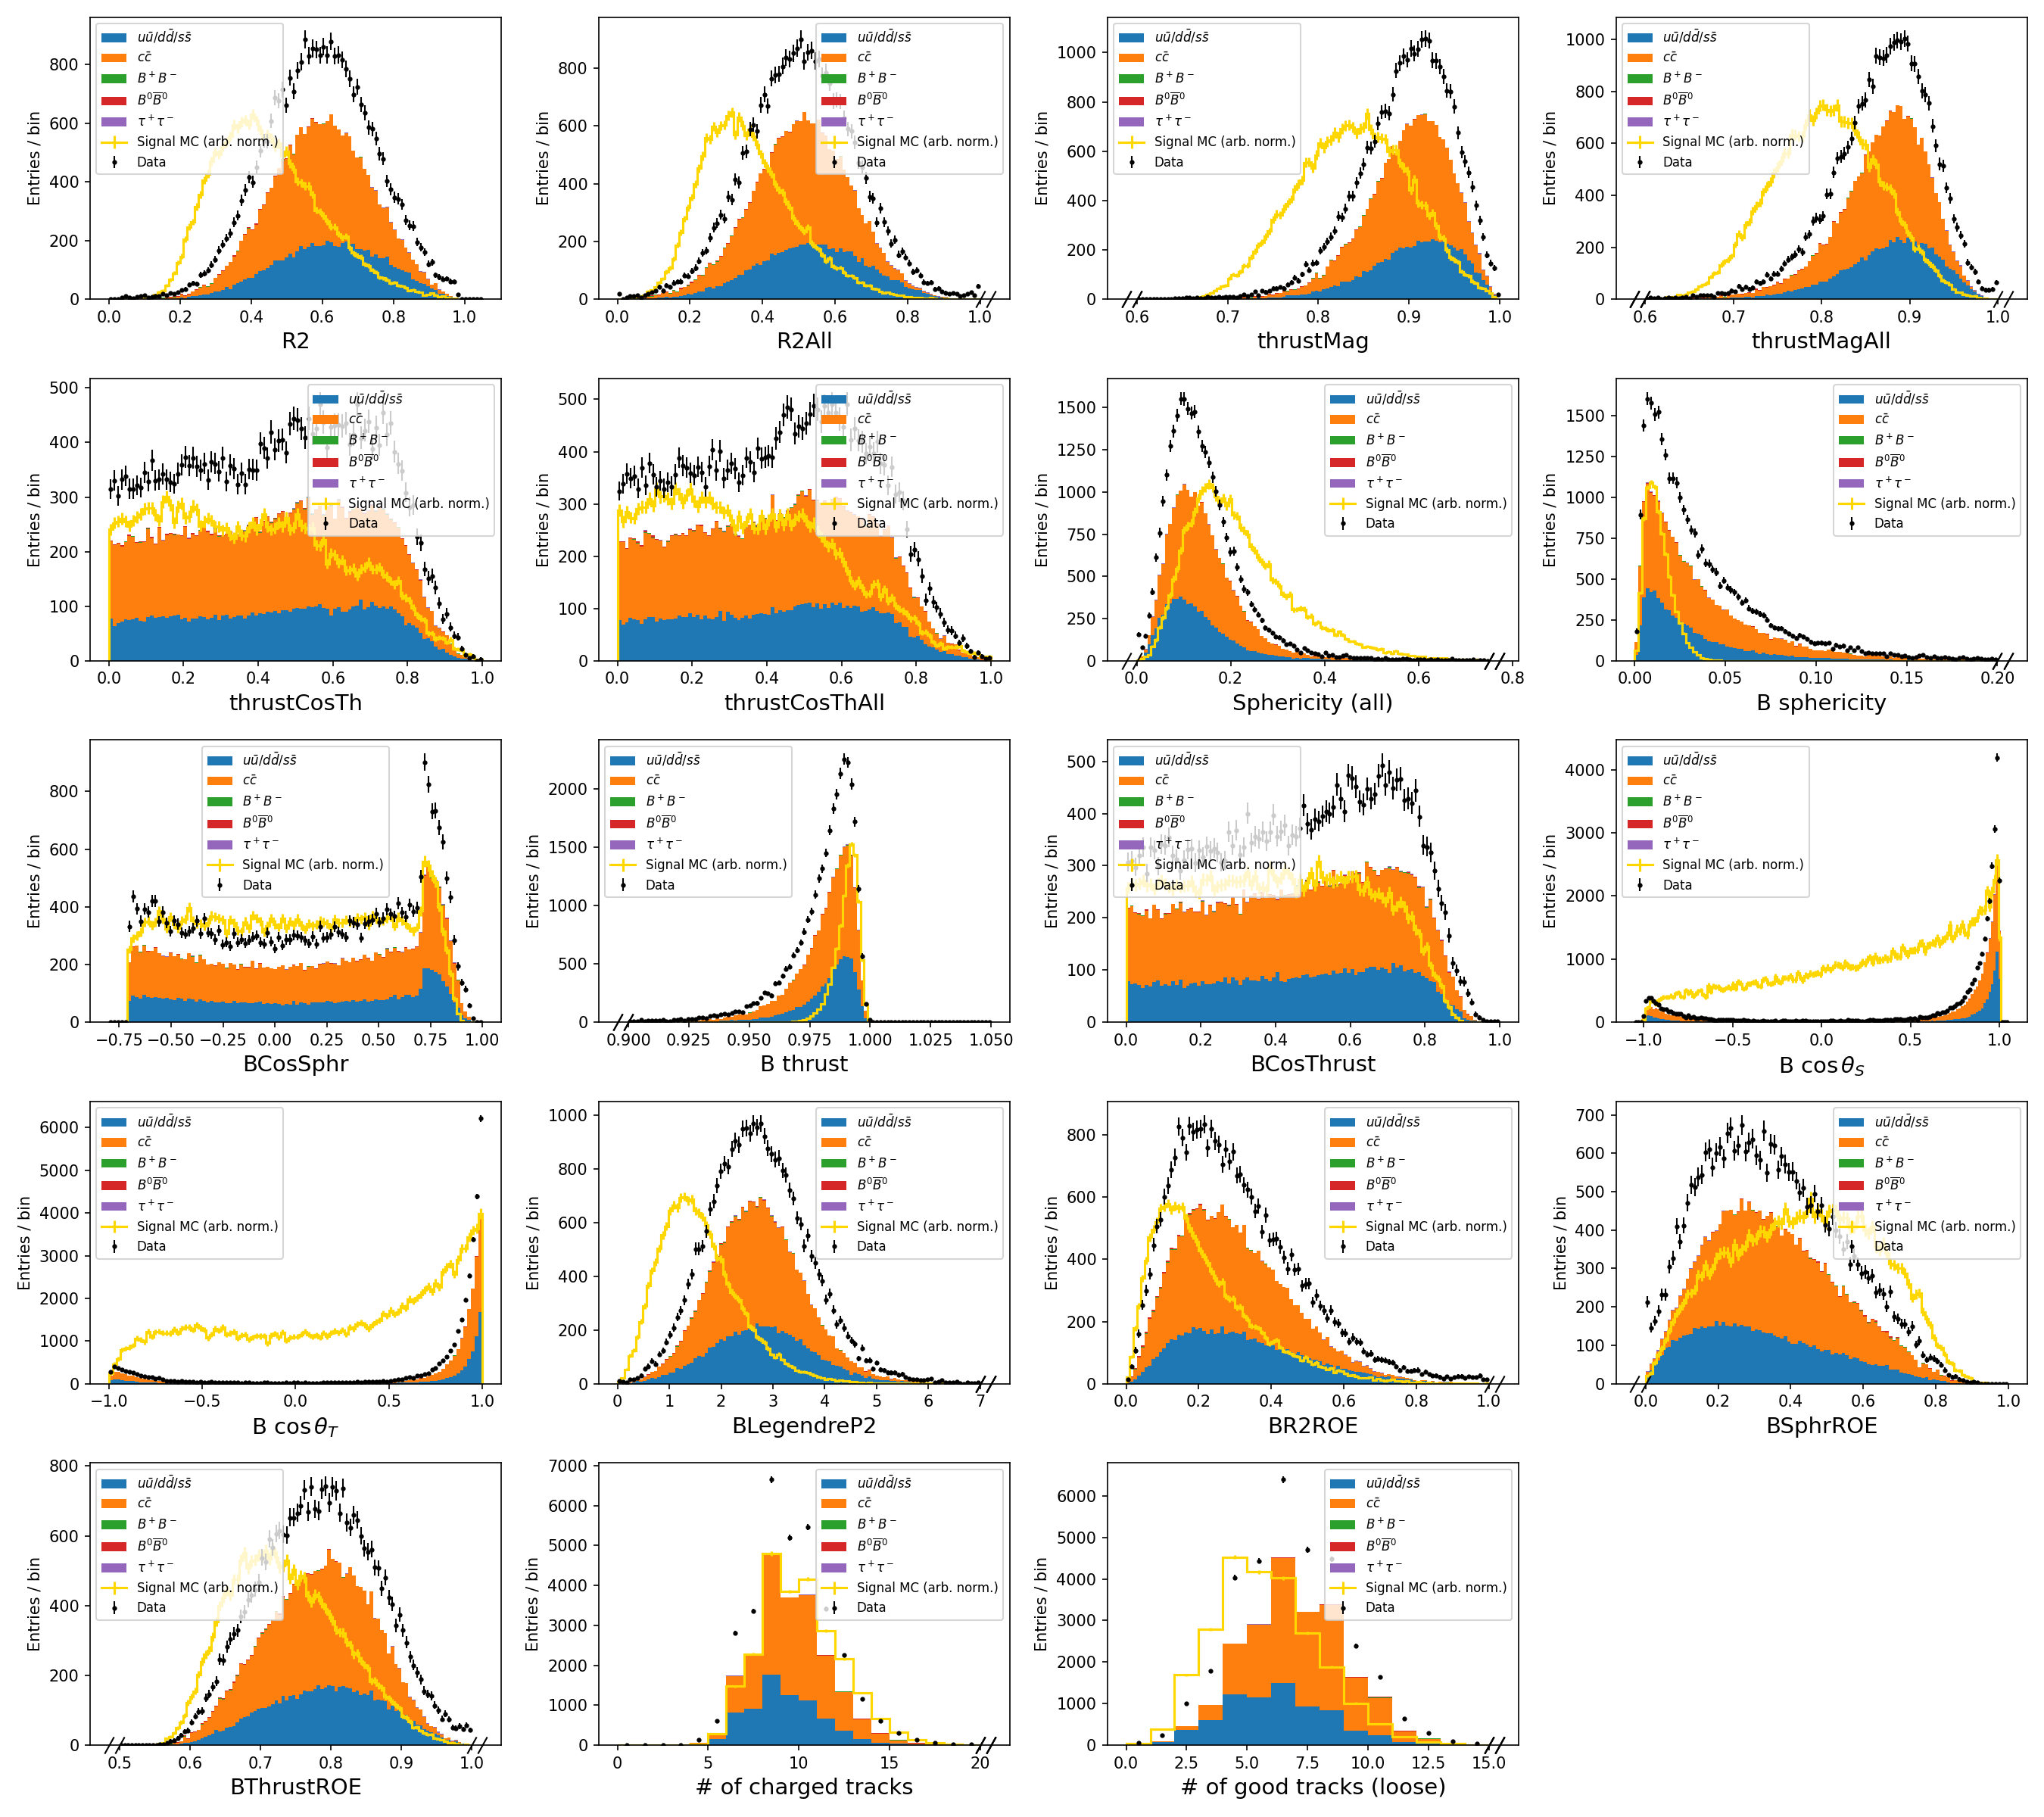
\includegraphics[width=0.99\textwidth]{figures/Lam0Lam0/diagnostics_cut1_eventshape.png}
    \caption{Event-shape variables for
    $\Bz \rightarrow \Lambda^0\Lambda^0$ after the single-candidate
    requirement.}
    \label{fig:eventshape_LamLam}
\end{figure}

\begin{figure}[tbp]
    \centering
    
\includegraphics[width=0.99\textwidth]{figures/Lam0LamC/diagnostics_cut1_eventshape.png}
    \caption{Same as Figure~\ref{fig:eventshape_LamLam} for
    $\Bu \rightarrow \Lambda_c^+\Lambda^0$.}
    \label{fig:eventshape_LamLamC}
\end{figure}

\subsection{$\Lambda^0$, $K_S^0$, and $\Lambda_c^+$ purity optimization
(Stage 2)\label{sec:stage2purity}}

All numbers and figures in this section use MC only (signal and
luminosity-weighted background) -- no collision data is examined, per the
blinding policy. The composite mass windows are re-optimized per channel
(rather than simply reused from the $\bar{p}\Lambda^0$ analysis) with an
$S/\sqrt{S+B}$ figure of merit: $S$ is the sideband-subtracted signal-MC
yield in the mass-peak window, and $B$ is the sideband-estimated background
from luminosity-weighted background MC, where the sideband bands are
contiguous with the peak window and have the same width as the peak. For
each composite ($\Lambda^0$, and, for $\Bu \rightarrow \Lambda_c^+\Lambda^0$,
$K_S^0$) the flight-significance cut is scanned first at the current mass
window, then the mass half-width is scanned with that flight cut applied.
$K_S^0$ is optimized \emph{before} $\Lambda_c^+$: it is a daughter of the
$\Lambda_c^+$ in decay modes 2 and 3, so its cut is fixed first and applied
as a gate (a no-op for modes 1 and 4) before the $\Lambda_c^+$ per-mode
windows are set. Recommended values that showed a genuine interior FOM
maximum have been applied to the analysis configuration (noted below as
each is discussed); values whose scan hit the edge of the scanned range
have not been, pending the methodology fix discussed below.

\begin{figure}[tbp]
    \centering
    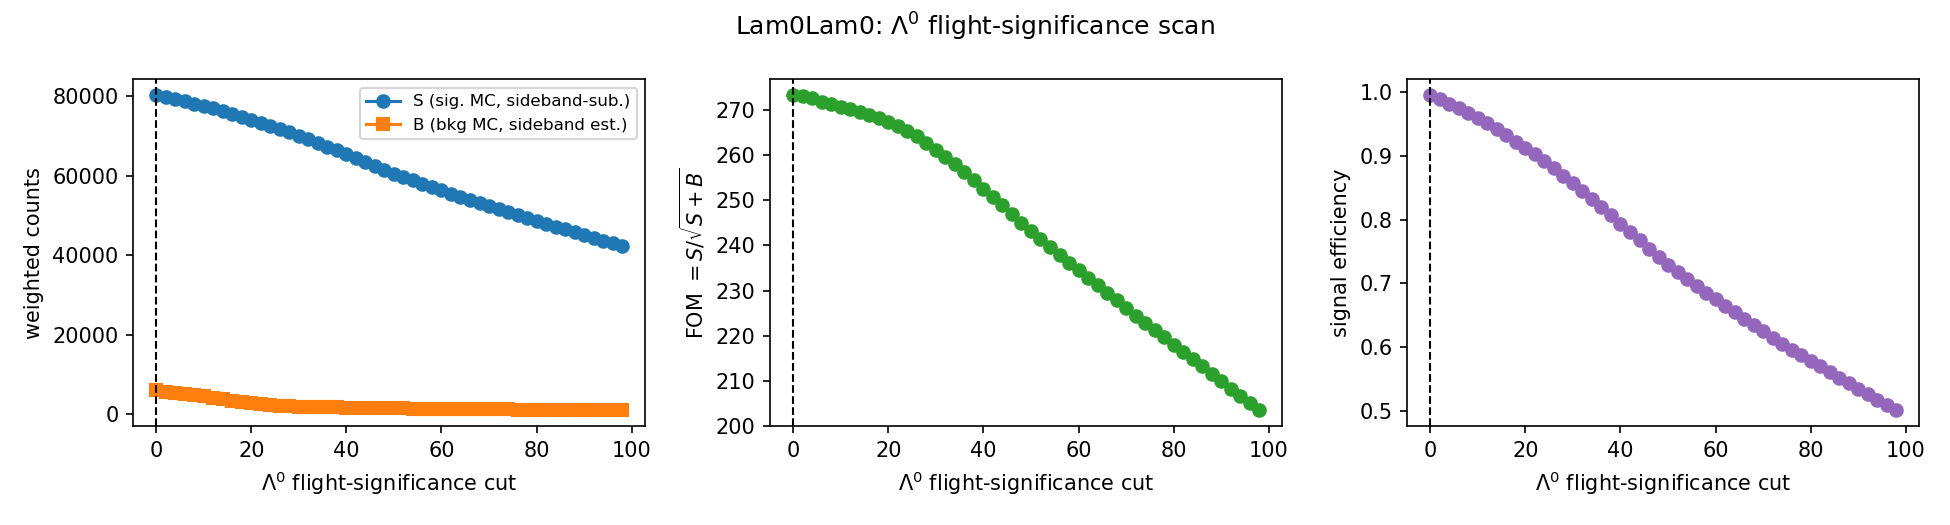
\includegraphics[width=0.99\textwidth]{figures/Lam0Lam0/lambda0_flight_scan.png}
    
\includegraphics[width=0.99\textwidth]{figures/Lam0LamC/lambda0_flight_scan.png}
    \caption{$\Lambda^0$ flight-significance $S/\sqrt{S+B}$ scan (mass
    window fixed at the current default) for $\Bz \rightarrow
    \Lambda^0\Lambda^0$ (top) and $\Bu \rightarrow \Lambda_c^+\Lambda^0$
    (bottom); the dashed line marks the scanned maximum.}
    \label{fig:lambda0_flight_scan}
\end{figure}

\begin{figure}[tbp]
    \centering
    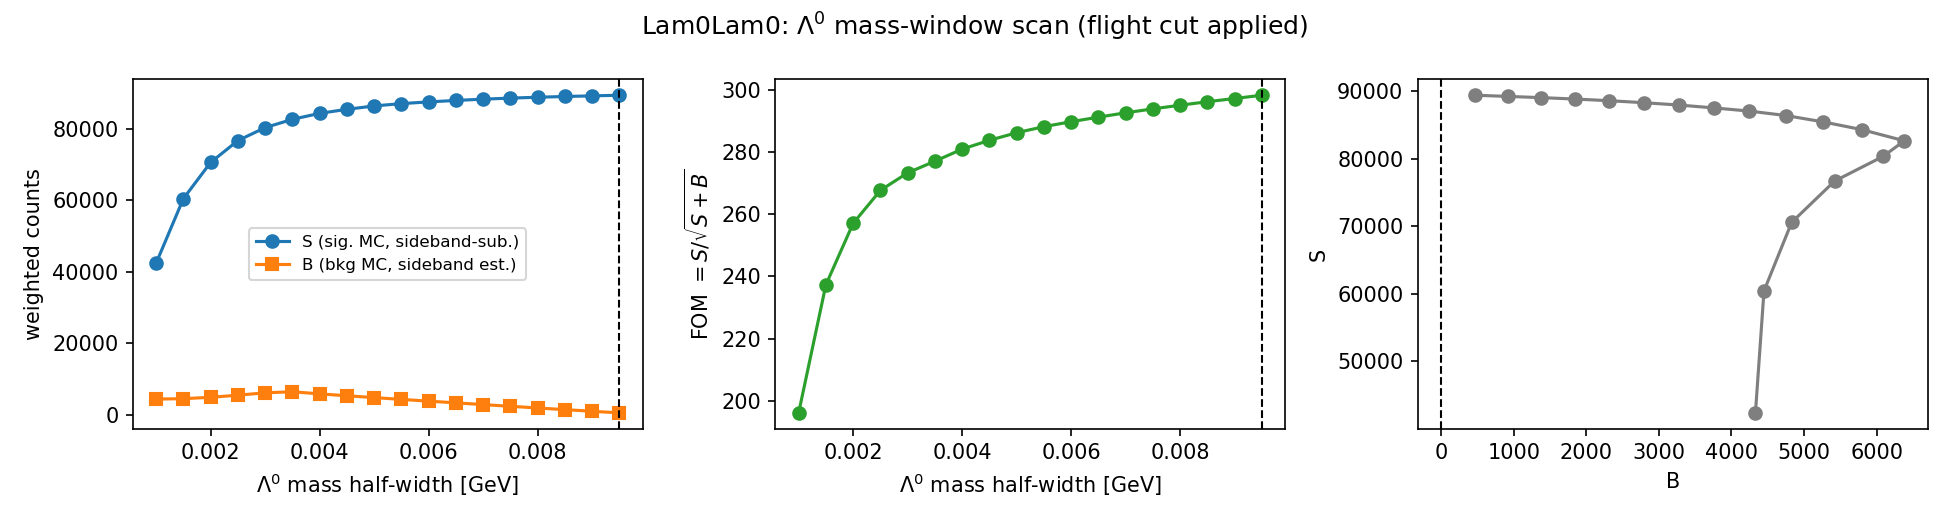
\includegraphics[width=0.99\textwidth]{figures/Lam0Lam0/lambda0_mass_scan.png}
    
\includegraphics[width=0.99\textwidth]{figures/Lam0LamC/lambda0_mass_scan.png}
    \caption{$\Lambda^0$ mass-half-width $S/\sqrt{S+B}$ scan (flight cut
    from Figure~\ref{fig:lambda0_flight_scan} applied), same channel
    ordering.}
    \label{fig:lambda0_mass_scan}
\end{figure}

For $\Bz \rightarrow \Lambda^0\Lambda^0$, the scanned optimum is
$>\LamLamLamZeroRecFlightSigCut$ for the flight significance and
$\pm\LamLamLamZeroRecMassWindowMeV$~MeV for the mass window; for
$\Bu \rightarrow \Lambda_c^+\Lambda^0$, $>\LamLamCLamZeroRecFlightSigCut$
and $\pm\LamLamCLamZeroRecMassWindowMeV$~MeV. \textbf{Both mass-window
scans, and the $\Lambda^0\Lambda^0$-channel flight-significance scan, are
at the edge of the scanned range} (Figures~\ref{fig:lambda0_flight_scan}
and~\ref{fig:lambda0_mass_scan}): the FOM is monotonic across the entire
grid rather than showing an interior maximum. The most likely explanation
is that the input ntuples are already skimmed to a narrow band around the
$\Lambda^0$ mass, so the sideband bands run out of background before the
scan range does, which biases $S/\sqrt{S+B}$ toward the widest/loosest
setting available rather than reflecting the true purity/efficiency
trade-off. The $\Lambda_c^+\Lambda^0$-channel $\Lambda^0$
flight-significance scan, by contrast, shows a genuine interior maximum at
$\LamLamCLamZeroRecFlightSigCut$ (Figure~\ref{fig:lambda0_flight_scan},
bottom) -- close to the $\bar{p}\Lambda^0$ default of 25 -- which is
evidence that the sideband method itself is sound, and \textbf{this value
has been applied} to \texttt{channel\_config.py}. The boundary-hugging cases
(both mass-window scans, and the $\Lambda^0\Lambda^0$-channel
flight-significance scan) have \textbf{not} been applied -- they remain at
the $\bar{p}\Lambda^0$ defaults pending either a wider mass-window scan
range or a methodology change (e.g.\ restricting the scan to candidates
already in the \mes/\DeltaE\ fitting region). \textbf{This is flagged for
review, not yet resolved.}

\begin{figure}[tbp]
    \centering
    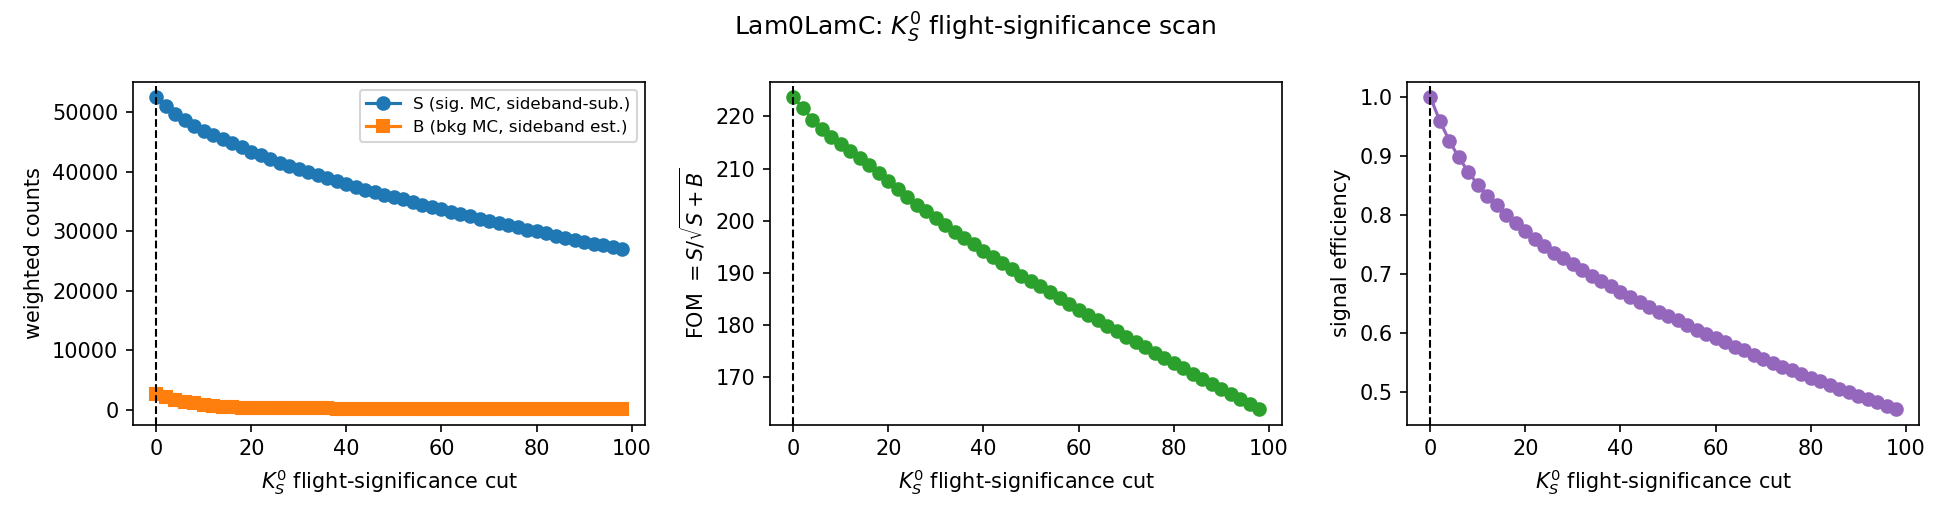
\includegraphics[width=0.85\textwidth]{figures/Lam0LamC/k0s_flight_scan.png}
    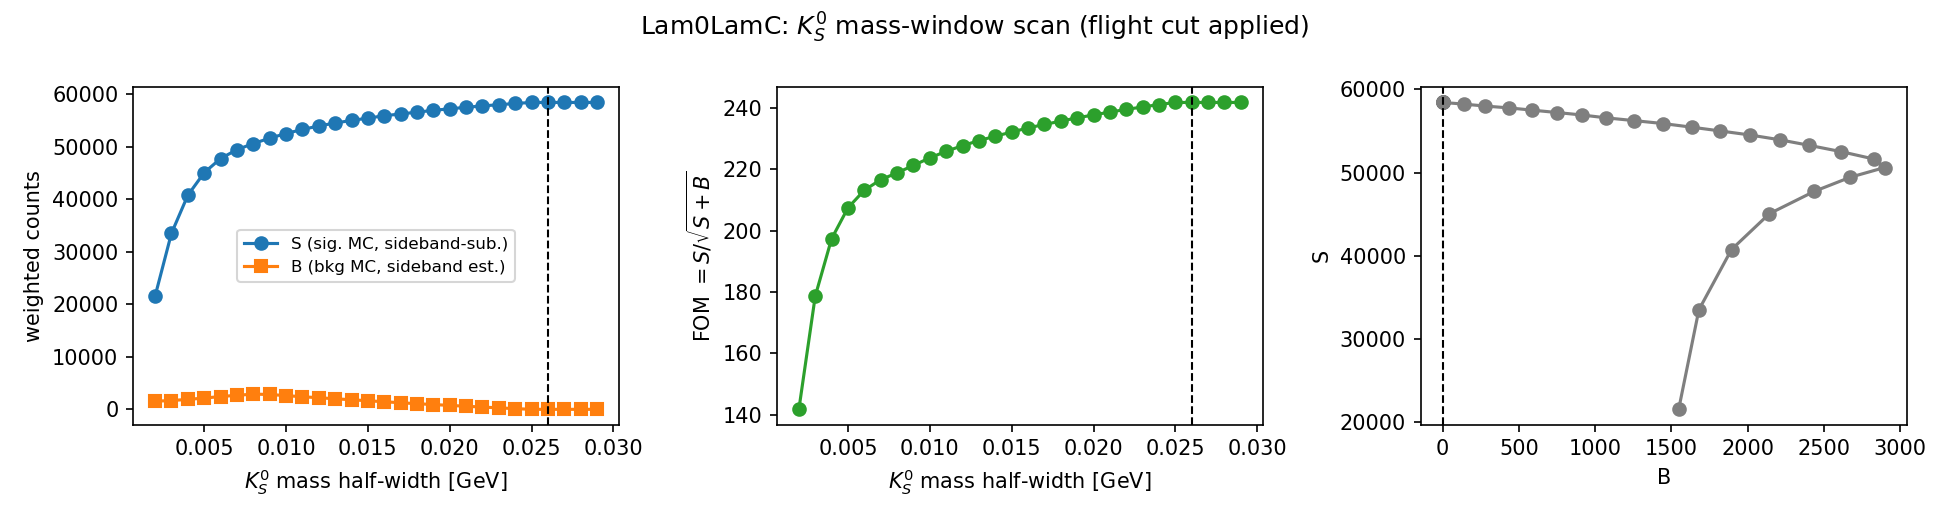
\includegraphics[width=0.85\textwidth]{figures/Lam0LamC/k0s_mass_scan.png}
    \caption{$K_S^0$ flight-significance (top) and mass-half-width (bottom)
    $S/\sqrt{S+B}$ scans, $\Bu \rightarrow \Lambda_c^+\Lambda^0$ channel.}
    \label{fig:k0s_scan}
\end{figure}

The $K_S^0$ scan (Figure~\ref{fig:k0s_scan}) shows the mirror-image
pattern: the mass-window scan gives an interior optimum of
$\pm\LamLamCKZeroRecMassWindowMeV$~MeV (consistent with the pre-fit $K_S^0$
mass resolution of order 8~MeV noted in Stage 1), which \textbf{has been
applied}; the flight-significance scan again hugs the scan boundary
($>\LamLamCKZeroRecFlightSigCut$) and has \textbf{not} been applied,
remaining at the Stage 1 placeholder pending the same methodology fix.

\begin{figure}[tbp]
    \centering
    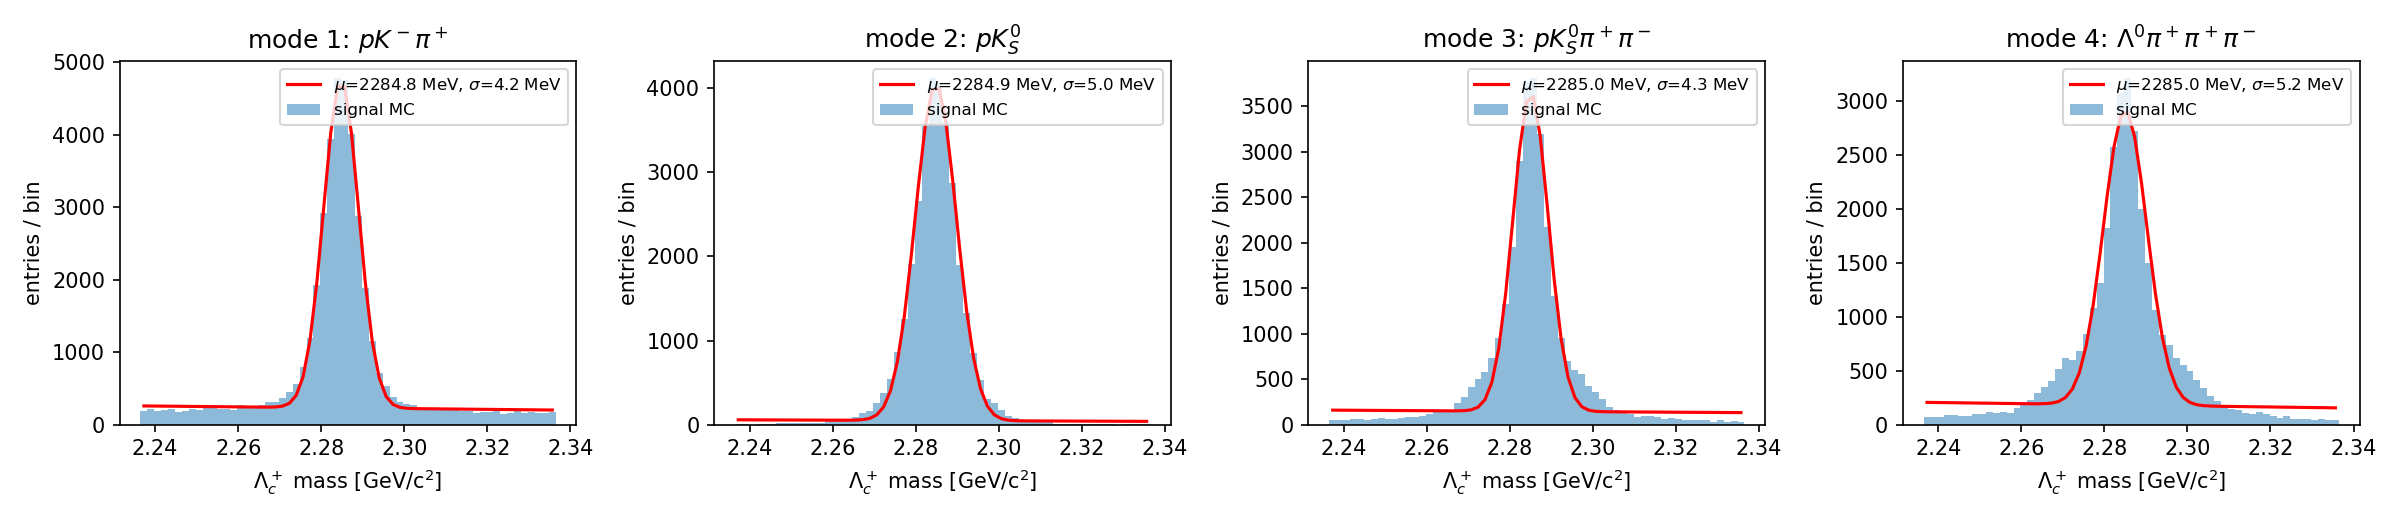
\includegraphics[width=0.99\textwidth]{figures/Lam0LamC/lambdac_mode_mass_fits.png}
    \caption{Per-mode $\Lambda_c^+$ mass fit (Gaussian + linear background,
    signal MC, recommended $K_S^0$ gate applied to modes 2 and 3).}
    \label{fig:lambdac_mode_fits}
\end{figure}

Unlike $\Lambda^0$ and $K_S^0$, the $\Lambda_c^+$ mass window is set from
the fitted per-mode resolution rather than an $S/\sqrt{S+B}$ scan: the
dominant ``background'' under the $\Lambda_c^+$ peak, even in signal MC
alone, is wrong-candidate combinatorics from the same signal event (up to
$\sim$60 $B$ candidates/event, Section~\ref{sec:lambdacmodes}), not a
separate smooth background process that a sideband can characterize.
Figure~\ref{fig:lambdac_mode_fits} shows the fit for each mode;
Table~\ref{tab:lambdacmodefits} gives the numbers. The window is
$\LamLamCLamCMassWindowNSigma\sigma$ around the fitted mean, chosen to keep
the great majority of the (near-Gaussian) core while still rejecting the
combinatorial tails visible in each panel; modes 2 and 4 (fewer or
different daughters) have a visibly worse resolution than modes 1 and 3.
\textbf{These four per-mode windows have been applied} to
\texttt{channel\_config.py}. Figure~\ref{fig:lambdac_before_after_k0s} confirms the
$\Lambda_c^+$ peak position and width in modes 2 and 3 are not meaningfully
changed by the $K_S^0$ gate (its mass window applied, its flight cut still
at the Stage 1 placeholder -- see above), so the sequential
$K_S^0$-then-$\Lambda_c^+$ optimization order is not sensitive to that
caveat.

% AUTO-GENERATED -- DO NOT EDIT BY HAND
\begin{table}[h]
\caption{Per-mode $\Lambda_c^+$ mass fit (Gaussian + linear background, signal MC, $K_S^0$ gate applied to modes 2 and 3) and the resulting mass\_window\_nsigma$\times\sigma$ window.}
\label{tab:lambdacmodefits}
\centering
\begin{tabular}{clrrrr}
\toprule
Mode & Decay & $\mu$ [MeV] & $\sigma$ [MeV] & converged & window [MeV] \\
\midrule
1 & $p K^- \pi^+$ & 2284.8 & 4.2 & yes & $\pm$12.6 \\
2 & $p K_S^0$ & 2284.9 & 5.0 & yes & $\pm$14.9 \\
3 & $p K_S^0 \pi^+ \pi^-$ & 2285.0 & 4.3 & yes & $\pm$12.8 \\
4 & $\Lambda^0 \pi^+ \pi^+ \pi^-$ & 2285.0 & 5.2 & yes & $\pm$15.7 \\
\bottomrule
\end{tabular}
\end{table}


\begin{figure}[tbp]
    \centering
    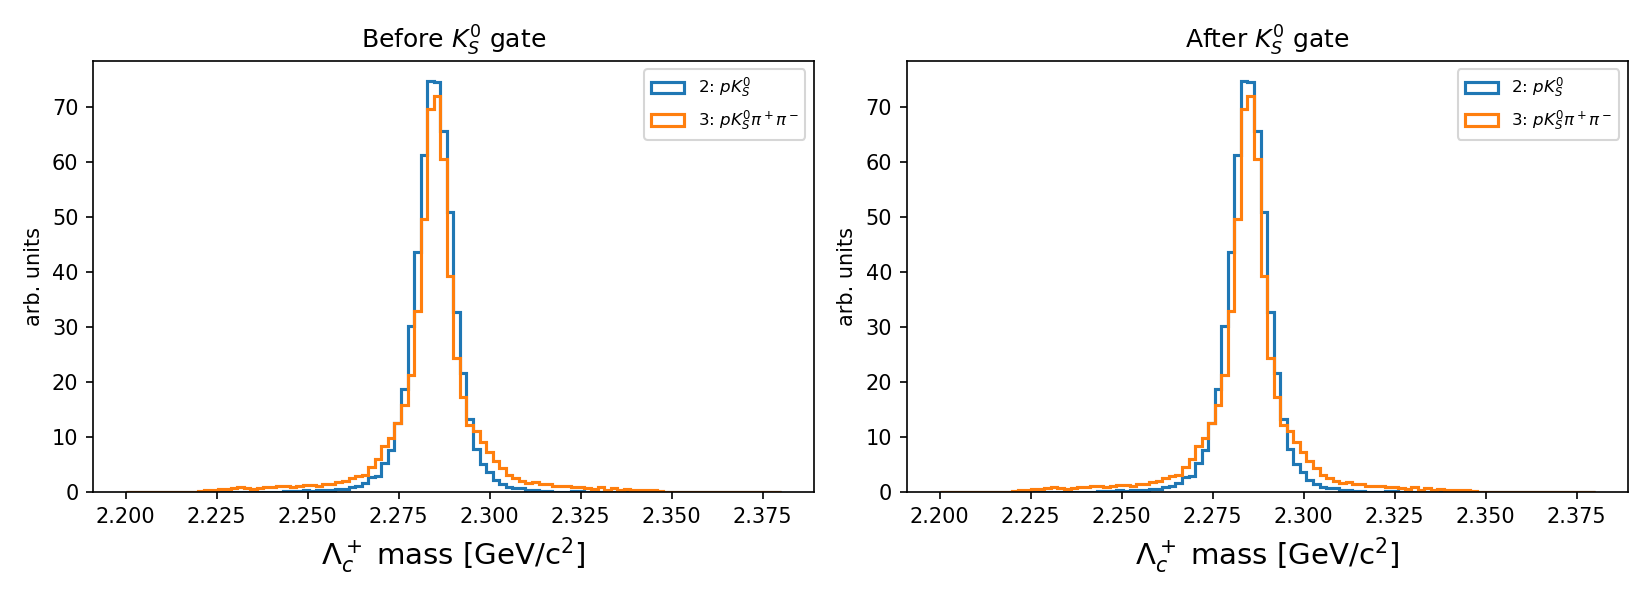
\includegraphics[width=0.85\textwidth]{figures/Lam0LamC/lambdac_mass_before_after_k0s_gate.png}
    \caption{$\Lambda_c^+$ mass, modes 2 and 3 only, before (left) and after
    (right) the recommended $K_S^0$ gate.}
    \label{fig:lambdac_before_after_k0s}
\end{figure}

Finally, Figure~\ref{fig:multicandidate} shows the number of $B$ candidates
per signal-MC event with \emph{both} composite daughters passing their
purity mask, after all cuts above (recommended values), for
$\Bu \rightarrow \Lambda_c^+\Lambda^0$: $\LamLamCFracZeroGoodBPct\%$ of
events have none, $\LamLamCFracOneGoodBPct\%$ have exactly one, and
$\LamLamCFracMultiGoodBPct\%$ still have more than one. This is a large
reduction in the multi-candidate rate from the Stage 1 baseline, but --
per the Stage 1 open decision (Section~\ref{sec:lambdacmodes}) -- no
candidate-selection policy is applied yet; that choice is deferred until
after the PID and antibaryon-veto stages.

\begin{figure}[tbp]
    \centering
    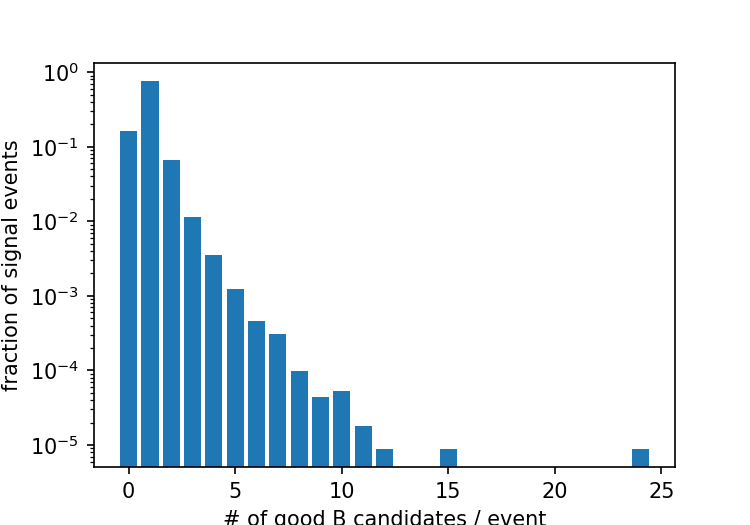
\includegraphics[width=0.6\textwidth]{figures/Lam0LamC/multi_candidate_study.png}
    \caption{Number of good $B$ candidates per signal-MC event after all
    Stage 2 purity cuts, $\Bu \rightarrow \Lambda_c^+\Lambda^0$.}
    \label{fig:multicandidate}
\end{figure}

\subsection{PID selector optimization (Stage 3)\label{sec:stage3pid}}

As in Section~\ref{sec:stage2purity}, all numbers and figures in this
section use MC only -- no collision data is examined. Charged-track PID
information is decoded from the per-track \texttt{<particle>SelectorsMap}
bitmaps (\texttt{pid\_selector.py}, ported from the $\bar{p}\Lambda^0$
analysis's \texttt{myPIDselector.py} and validated bit-for-bit against it)
and optimized with the Punzi figure of merit appropriate to an upper-limit
search~\cite{Punzi:2003bu}: $\mathrm{FOM} = \epsilon_{\rm sig}/\sqrt{B + a/2}$
with $a=4$, where $\epsilon_{\rm sig}$ is the signal-MC efficiency of the PID
cut \emph{relative to} the Stage 1/2 selection already in force, and $B$ is
the luminosity-weighted count of background MC (all SP modes, not the two
ad hoc continuum modes used in the $\bar{p}\Lambda^0$ reference) surviving
the same selection directly in the \mes/\DeltaE\ signal region -- an
MC-truth background estimate, not the sideband-based one used in
Section~\ref{sec:stage2purity} (a data-driven sideband estimate is deferred
to Stage 5/6). The scan is over the KM-family selector ladder (Super Loose
through Super Tight) for each PID target: the $\Lambda^0$ proton and pion
daughters (both channels, and reused for $\Lambda_c^+$ mode 4's embedded
$\Lambda^0$ rather than re-scanned); and, for $\Bu \rightarrow
\Lambda_c^+\Lambda^0$, each $\Lambda_c^+$ decay mode's own daughters, scanned
independently per mode since the relevant particles differ by mode (mode 1:
$p$, $K^-$, $\pi^+$; mode 2: $p$ only; mode 3: $p$, $\pi^\pm$; mode 4: the
three $\pi^\pm$ daughters, with the embedded $\Lambda^0$ covered by the
$\Lambda^0$ scan above). No PID cut is applied to the $K_S^0$'s own $\pi^+\pi^-$
daughters at this stage (deferred as a possible future refinement).
\textbf{None of the values in this section have been applied to
\texttt{channel\_config.py} yet} -- Stage 3 produces recommendations for
review, exactly as Stage 2 did.

\begin{figure}[tbp]
    \centering
    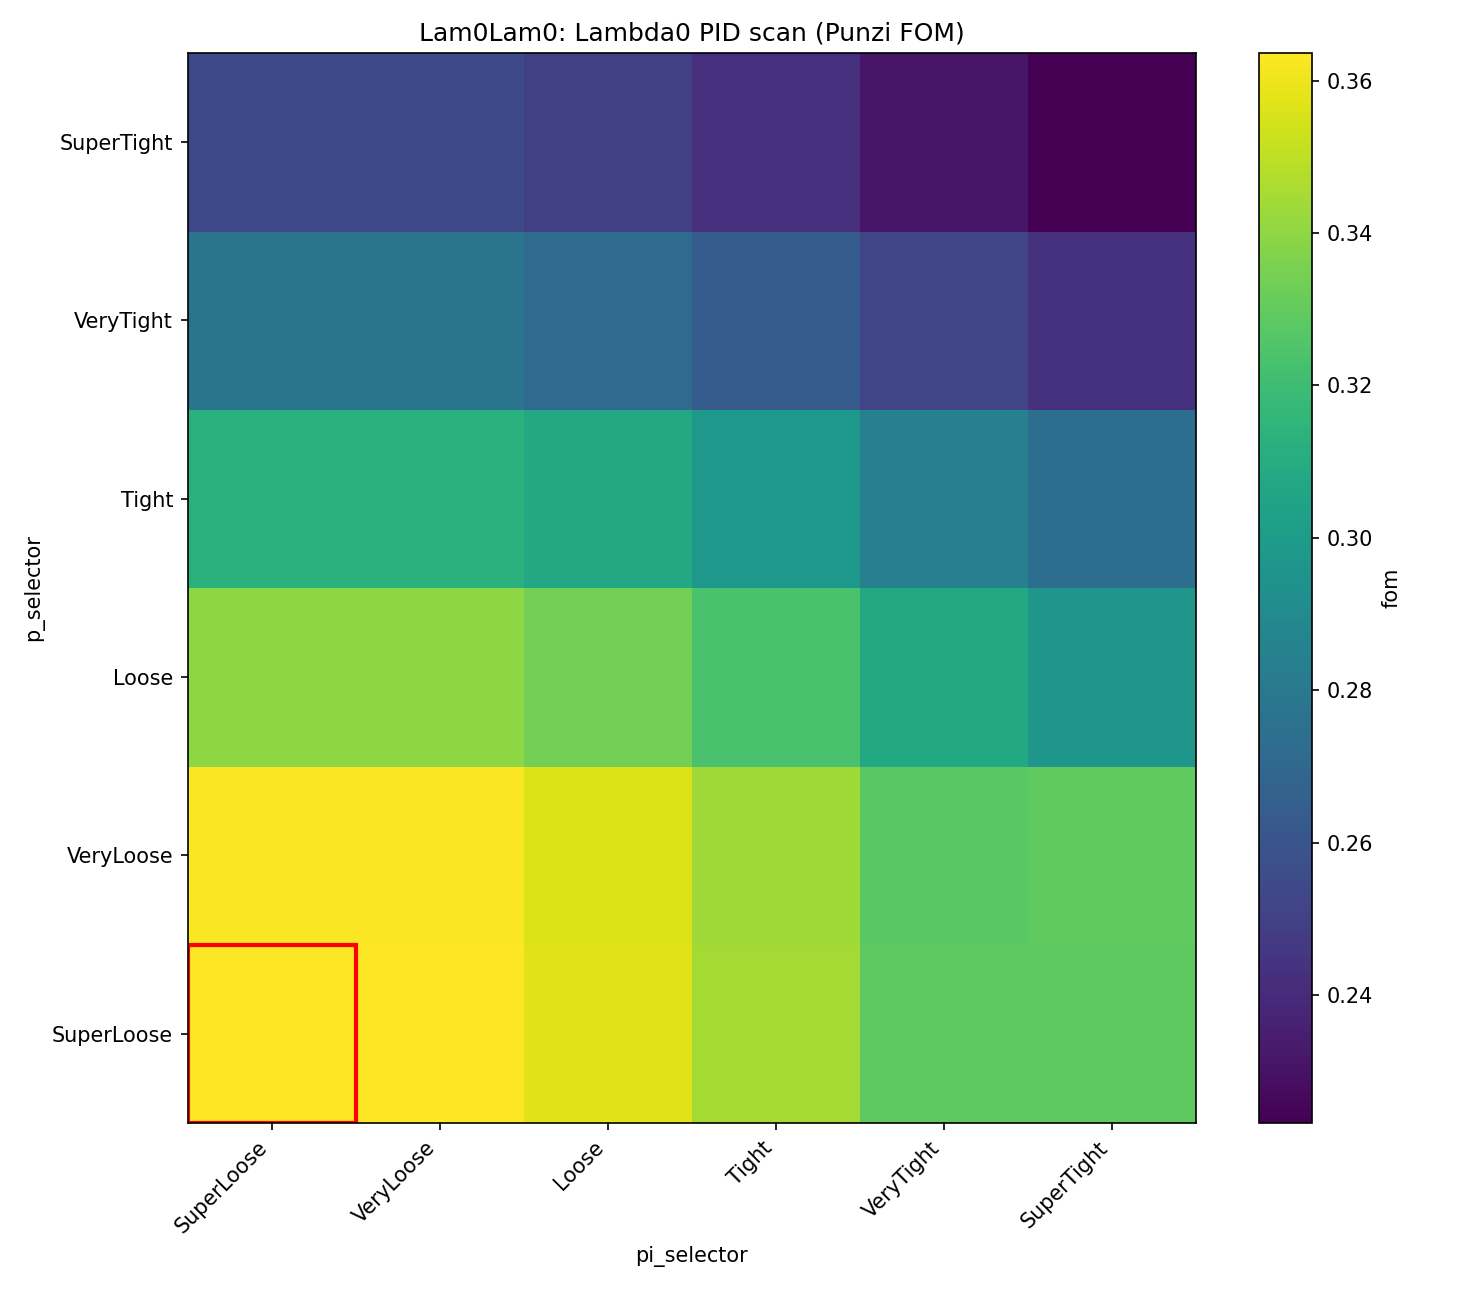
\includegraphics[width=0.62\textwidth]{figures/Lam0Lam0/lambda0_pid_scan.png}
    
\includegraphics[width=0.62\textwidth]{figures/Lam0LamC/lambda0_pid_scan.png}
    \caption{$\Lambda^0$ proton $\times$ pion Punzi-FOM PID scan for $\Bz
    \rightarrow \Lambda^0\Lambda^0$ (top) and $\Bu \rightarrow
    \Lambda_c^+\Lambda^0$ (bottom); the boxed cell marks the scan maximum.}
    \label{fig:lambda0_pid_scan}
\end{figure}

Table~\ref{tab:pidselectors} summarizes every scan's recommended
selector(s), FOM, efficiency, background, and whether the optimum sits at
the edge of the scanned ladder rather than at a genuine interior maximum
(as in Section~\ref{sec:stage2purity}, this is flagged rather than silently
trusted). A second, PID-specific failure mode is also checked at every grid
point: a tight enough selector can drive the weighted background estimate
toward zero on very few raw MC candidates, inflating the FOM from a noisy
denominator rather than real background rejection; none of the recommended
operating points triggered this (raw background-MC candidate counts at the
recommended cut ranged from 6 to 333 across all scans).

% AUTO-GENERATED -- DO NOT EDIT BY HAND
\begin{table}[h]
\caption{Stage 3 recommended KM-ladder PID selector(s), the Punzi FOM ($a=4$) and signal efficiency/background at that operating point, and whether the scan optimum sits at the edge of the scanned ladder (see text before applying).}
\label{tab:pidselectors}
\centering
\small
\resizebox{\textwidth}{!}{%
\begin{tabular}{lp{5.5cm}rrrc}
\toprule
Target & Recommended selector(s) & FOM & $\epsilon_{sig}$ [\%] & $B$ (wtd.) & boundary? \\
\midrule
$B^0 \to \Lambda^0 \Lambda^0$: $\Lambda^0$ & p: SuperLoose, pi: SuperLoose & 0.364 & 92.8 & 4.51 & yes \\
$B^+ \to \Lambda_c^+ \Lambda^0$: $\Lambda^0$ & p: SuperLoose, pi: SuperLoose & 0.082 & 96.8 & 135.97 & yes \\
$B^+ \to \Lambda_c^+ \Lambda^0$: $\Lambda_c^+$ mode 1 ($p K^- \pi^+$) & K: VeryLoose, p: Tight, pi: SuperLoose & 0.438 & 90.3 & 2.24 & yes \\
$B^+ \to \Lambda_c^+ \Lambda^0$: $\Lambda_c^+$ mode 2 ($p K_S^0$) & p: Loose & 0.449 & 92.6 & 2.25 & no \\
$B^+ \to \Lambda_c^+ \Lambda^0$: $\Lambda_c^+$ mode 3 ($p K_S^0 \pi^+ \pi^-$) & p: SuperTight, pi: SuperLoose & 0.419 & 88.7 & 2.49 & yes \\
$B^+ \to \Lambda_c^+ \Lambda^0$: $\Lambda_c^+$ mode 4 ($\Lambda^0 \pi^+ \pi^+ \pi^-$) & pi: SuperLoose & 0.263 & 95.6 & 11.18 & yes \\
\bottomrule
\end{tabular}
}
\end{table}


\textbf{The $\Lambda^0$ scan is boundary-hugging (loosest rung) in both
channels} (Figure~\ref{fig:lambda0_pid_scan}): unlike
Section~\ref{sec:stage2purity}'s boundary-hugging cases (traced to an
upstream mass-skim depleting the sidebands), the likely explanation here is
simpler -- the background already surviving the Stage 1/2 purity cuts, in
the signal region, is low enough that any efficiency lost by tightening PID
further is not worth the marginal background rejection. An explicit check
against applying \emph{no} PID cut at all confirms the recommended (loosest)
selector is still a genuine, if modest, improvement over no cut
(FOM~$\LamLamLamZeroPidFom$ vs.\ $\LamLamLamZeroPidFomNoPidAtAll$ for
$\Bz\to\Lambda^0\Lambda^0$; $\LamLamCLamZeroPidFom$ vs.\
$\LamLamCLamZeroPidFomNoPidAtAll$ for $\Bu\to\Lambda_c^+\Lambda^0$, a much
smaller margin) -- so the true optimum plausibly lies outside the KM ladder
entirely, at an even looser (or no) requirement, rather than at a real
trade-off within it.

The four $\Lambda_c^+$ per-mode scans are more mixed. Mode 2 ($pK_S^0$)
gives a genuine interior optimum (Loose proton) -- the one clean result,
echoing Section~\ref{sec:stage2purity}'s single clean scan. Mode 1
($pK^-\pi^+$, Figure~\ref{fig:lambdac_mode1_pid_scan}) is a partial success:
the proton and kaon dimensions both land on clean interior optima (Tight
proton, Very Loose kaon), while the pion dimension still prefers the
loosest rung. Modes 3 and 4 are boundary-hugging in every scanned dimension;
mode 3 is notable for pulling in \emph{opposite} directions (proton wants
the \emph{tightest} rung, pion the \emph{loosest}), suggestive of a
proton-fake-dominated background in that mode, not yet investigated further.

\begin{figure}[tbp]
    \centering
    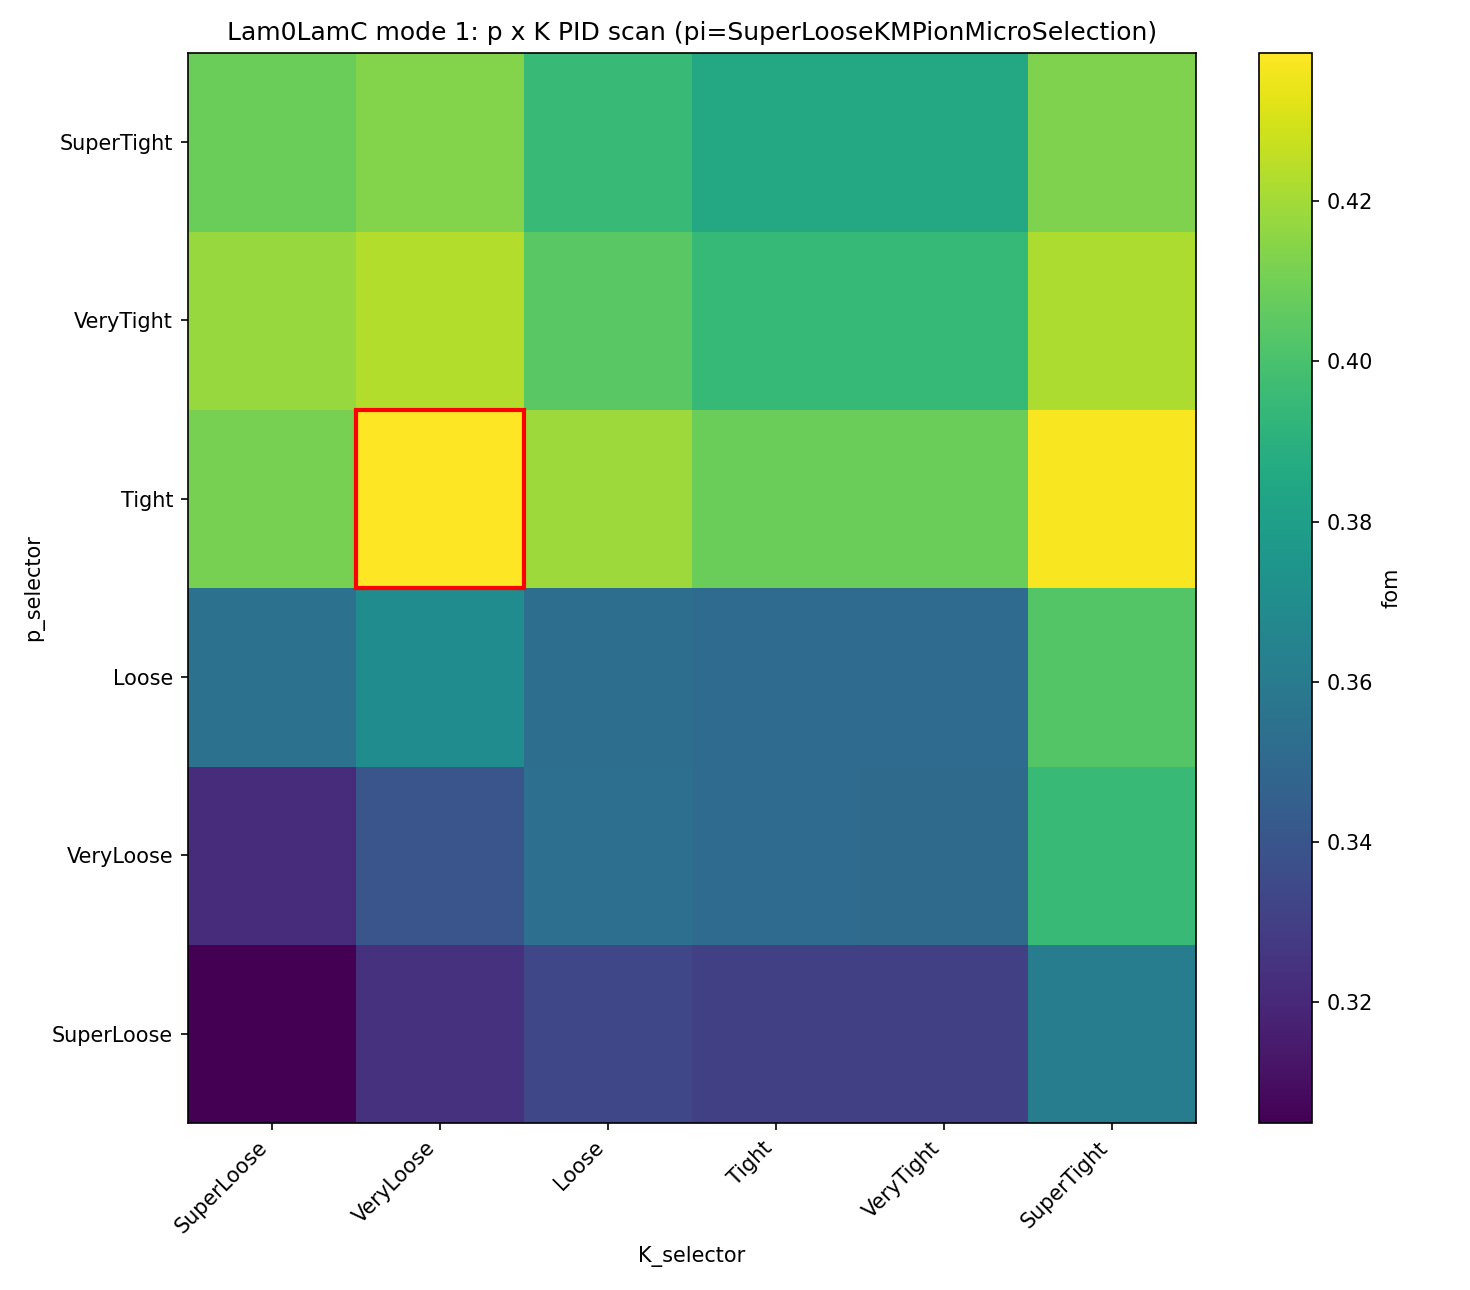
\includegraphics[width=0.75\textwidth]{figures/Lam0LamC/lambdac_mode1_pid_scan.png}
    \caption{$\Lambda_c^+$ mode 1 proton $\times$ kaon Punzi-FOM PID scan
    (pion selector fixed at its own recommended value).}
    \label{fig:lambdac_mode1_pid_scan}
\end{figure}

Redoing the Section~\ref{sec:stage2purity} multi-candidate study with these
recommended PID selectors folded in on top of the Stage 2 purity cuts (
$\Bu \rightarrow \Lambda_c^+\Lambda^0$): the good-$B$-candidate fractions
move from ($\LamLamCFracZeroGoodBPct\%$, $\LamLamCFracOneGoodBPct\%$,
$\LamLamCFracMultiGoodBPct\%$) to ($\LamLamCFracZeroGoodBPidPct\%$,
$\LamLamCFracOneGoodBPidPct\%$, $\LamLamCFracMultiGoodBPidPct\%$) for
(0, 1, $>$1) good candidates. PID removes a sizeable fraction of previously
good candidates outright -- mostly via the $\Lambda_c^+$ per-mode cuts,
since the $\Lambda^0$ selector is the loosest KM rung and costs little on
its own -- and reduces the multi-candidate fraction somewhat, but does not
resolve it. As in Section~\ref{sec:stage2purity}, this is \textbf{presented
for review, not a candidate-selection decision}: that choice remains
deferred (Section~\ref{sec:lambdacmodes}, open decision) until after the
antibaryon-veto stage.

Given how many of the scans above are boundary-hugging at the loosest KM
rung, the recommendation for the next checkpoint is to decide, per target,
whether ``no PID cut'' is preferable to ``loosest KM selector'' rather than
mechanically applying the ladder's edge value -- particularly for the
$\Lambda^0$ daughters and $\Lambda_c^+$ modes 3/4's pions.
